\section{Softwarearchitektur und Softwarekomponenten}
\label{sec:2_Architektur}
Das Kapitel \ref{sec:2_Architektur} sollte der Leserin und dem Leser verhelfen, den Begriff \glqq Softwarearchitektur\grqq\ zu verstehen. Demnach sollen Vorteile von der Verwendung von Softwarearchitektur genannt werden. Des Weiteren werden wichtige Begriffe wie serviceorientierte Architektur beziehungsweise komponentenbasierte Architektur näher erläutert.
Des Weiteren wird in Kapitel \ref{sec:2_Architektur} nur Architektur behandelt, die sich über die Erstellung, Auslieferung und den Betrieb von Software jeglicher Art erstreckt. Folglich gibt es Berührungspunkte zu anderen Architektur-Disziplinen wie zum Beispiel der Daten- oder Sicherheitsarchitektur, die jedoch nicht in dieser Arbeit behandelt werden.

\subsection{Klassische Softwarekomponente}
\label{sec:2_Softwarekomponente_Klassisch}
\begin{quote}
\glqq The characteristic properties of a component are that it:
\begin{itemize}
\item is a unit of independent deployment
\item is a unit of third-party composition
\item has no (externally) observable state\grqq
\end{itemize}
\end{quote}

Dies ist die Definition einer Komponente von Clemens Szyperski im Buch \glqq Component software: Beyond object-oriented programming\grqq \citereset \autocite{Szyperski.2002}.
Diese Definition bedarf weiterer Erläuterung.
\begin{description}
\item[A component is a unit of independent deployment] \hfill \\
Dieser Punkt der Definition besitzt eine softwaretechnische Implikation. Damit eine Komponente \glqq independent deployable\grqq\ also unabhängig auslieferbar ist, muss sie auch so konzipiert beziehungsweise entwickelt werden. Sämtliche Funktionen der Komponente müssen vollständig unabhängig von der Verwendungsumgebung und von anderen Komponenten sein. Des Weiteren muss der Begriff \glqq independent deployable\grqq\ als Ganzes betrachtet werden, denn es bedeutet, dass eine Komponente nicht partiell, sondern nur als Ganzes ausgeliefert wird. Ein Beispiel für diesen Kontext wäre, dass ein Dritter keinen Zugriff auf die involvierten Komponenten einer Software hat.\\
\item[A component is a unit of third-party composition] \hfill \\
Hier wird der Begriff \glqq composable\grqq\ dahingehend verstanden, dass Komponenten zusammensetzbar sein sollen. In diesem Kontext bedeutet dies, dass eine Applikation aus mehreren Komponenten bestehen kann. Des Weiteren soll auch mit einer Komponente interagiert werden können, was einer klar definierten Schnittstelle bedarf. Nur mit Hilfe dieser Schnittstelle kann garantiert werden, dass die Komponente einerseits vollständig gekapselt von anderen Komponenten ist und andererseits mit der Umgebung interagieren kann. Dies erfordert demnach eine klare Spezifikation, was die Komponente erfordert und was sie bietet.
\item[A component has no (externally observable) state] \hfill \\
Eine Komponente sollte keinen (externen) \glqq observable\grqq also feststellbaren Zustand haben. Die Originalkomponente darf nicht von Kopien ihrer selbst unterschiedlich sein. Wenn Komponenten einen feststellbaren Zustand haben dürften, wäre es nicht möglich, zwei \glqq gleiche\grqq\ Komponenten mit den gleichen Eigenschaften zu haben. Eine mögliche Ausnahme von dieser Regel sind Attribute, die nicht zur Funktionalität der Komponente beitragen. Ein Beispiel in diesem Kontext wäre die Seriennummer für die Buchhaltung. Dieser spezifische Ausschluss ermöglicht einen zulässigen technischen Einsatz eines Zustands, der kritisch für die Leistung sein könnte. Beispielsweise dafür sei der Cache. Eine Komponente kann einen Zustand mit der Absicht zu cachen verwenden. \todo{umschreiben!}Ein Cache ist ein Speicher, auf den man ohne Konsequenzen verzichten kann, jedoch möglicherweise reduzierte Leistung in Anspruch nimmt.
\end{description}

In vielen aktuellen Ansätzen sind Komponenten eine schwerwiegende Einheit mit genau einer Instanz in einem System. Beispielsweise könnte ein Datenbankserver eine Komponente darstellen. Oftmals wird der Datenbankserver im Zusammenhang mit der Datenbank als Modul mit einem feststellbaren Zustand angesehen. Dahingehend ist der Datenbankserver ein Beispiel für eine Komponente und die Datenbank ein Beispiel für das Objekt, das von der Komponente verwaltet wird. Es ist wichtig zwischen dem Komponentenkonzept und dem Objektkonzept zu differenzieren, da das Komponentenkonzept in keinster weise den Gebrauch von Zuständen von Objekten fördert beziehungsweise zurückstuft \citereset \autocite{Szyperski.2002}.

Eine Softwarearchitektur ist die zentrale Grundlage einer skalierbaren Softwaretechnologie und ist für komponentenbasierte Systeme von größter Bedeutung. Nur da, wo eine Gesamtarchitektur mit Wartbarkeit definiert ist, finden Komponenten die Grundlage, die sie benötigen. Folgend werden einige Eckpfeiler einer Komponentenarchitektur genannt \citereset \autocite{Szyperski.2002}:
\begin{itemize}
\item Interaktionen zwischen Komponenten und deren Umfeld sind geregelt
\item Die Rollen von Komponenten sind definiert
\item Schnittstellen von Komponenten sind standardisiert
\item Aspekte der Benutzeroberflächen für Endbenutzer und Assembler sind geregelt
\end{itemize}
In Kapitel \ref{sec:2_Softwarearchitektur} auf Seite \pageref{sec:2_Softwarearchitektur} wird der Begriff der Softwarearchitektur näher erläutert. Des Weiteren werden in Kapitel \ref{sec:2_Serviceorientierte_Softwarearchitektur} auf Seite \pageref{sec:2_Serviceorientierte_Softwarearchitektur} und Kapitel \ref{sec:2_Komponentenbasierte_Softwarearchitektur} auf Seite \pageref{sec:2_Komponentenbasierte_Softwarearchitektur} zwei Aspekte der Softwarearchitektur hinsichtlich der Entwicklung mit Komponenten erklärt.



\subsection{Arten von Softwarekomponenten}
\label{sec:2_Arten_Komponenten}

Verschiedene Arten von Komponenten können entsprechend ihren Aufgabenbereichen klassifiziert werden. Eine übersichtliche Art der Zuordnung von Aufgabenbereichen zu Komponenten kann auf der Basis der Trennung von Zuständigkeiten erfolgen, zum Beispiel auf der Basis einer Schichten-Architektur. Eine Schichtenarchitektur dient der Trennung von Zuständigkeiten und einer losen Kopplung der Komponenten. Sie unterteilt ein Software-System in mehrere horizontale Schichten, wobei das Abstraktionsniveau der einzelnen Schichten von unten nach oben zunimmt. Eine jede Schicht bietet der über ihr liegenden Schicht Schnittstellen an, über die diese auf sie zugreifen kann. Abbildung \ref{fig:2_Schichtenarchitektur} auf Seite \pageref{fig:2_Schichtenarchitektur} veranschaulicht die bereits genannte Architektur \citereset \autocite{Andresen.2003}.
\begin{figure}[h]
\centering
%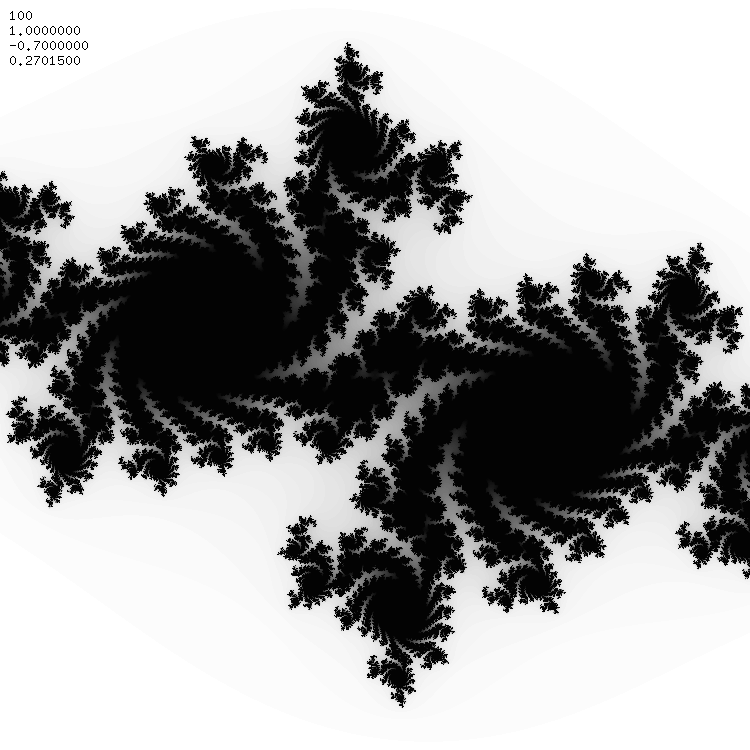
\includegraphics[height=5.0cm]{images/Julia-Fractal.png}
\missingfigure{Schichtenarchitektur}
\caption[
Beispiel einer Schichtenarchitektur, Urldate: 04.2014 \newline
%\small\texttt{http://upload.wikimedia.org/wikipedia/commons/e/e1/SchichtenarchitekturAufrufstrukturen.svg}
]{Beispiel einer Schichtenarchitektur}
\label{fig:2_Schichtenarchitektur}
\end{figure}





Auf Grundlage der in Abbildung \ref{fig:2_Schichtenarchitektur} auf Seite \pageref{fig:2_Schichtenarchitektur} veranschaulichten Architektur können Komponenten wie folgt unterteilt werden:
\begin{description}
\item[Komponenten der Präsentations-Schicht] \hfill \\
Diese Komponenten stellen eine nach außen sichtbare Benutzerschnittstelle dar. Ein Beispiel dieser Schnittstelle ist eine GUI\footnote{Graphical User Interface}-Komponente (Button, Menü, Slider, und vieles mehr\ldots).
\item[Komponenten der Controlling-Schicht] \hfill \\
Diese verarbeiten komplexe Ablauflogik und dienen als Vermittler zwischen Komponenten der Business- und Präsentations-Schicht.Beispielhaft hierfür wäre ein Workflow-Controller. Er koordiniert die Interaktion mit einer oder mehreren Businesskomponenten. Diese Komponente kann zum Beispiel den Ablauf eines Geschäftsprozesses umsetzen.
\item[Komponenten der Business-Schicht] \hfill \\
Sie bilden die Geschäftslogik im Sinne autonomer Businesskonzepte ab. Geschäftslogik in diesem Kontext bedeutet, dass die Komponente die Logik besitzt, die die eigentliche Problemstellung löst. Oftmals bezeichnet man hier die sogenannte Entity-Komponente. Sie dient der Perstistierung von Daten beziehungsweise bildet Entitäten auf Komponenten ab (Firma, Produkt, Kunden).
\item[Komponenten der Integrations-Schicht] \hfill \\
Sie dient der Anbindung an Alt-Systeme, Fremd-Systeme und Datenspeicher. Dies könnten eispielsweise Connector-Komponenten oder Datenzugriffs-Komponenten sein. Connector-Komponenten dienen der Integration eines Fremd-Systems und Datenzugriffs-Komponenten liefert den Datenzugriff für Komponenten der oben genannten Schichten. Bei Datenzugriffs-Komponenten werden die Besonderheiten einer Datenbank berücksichtigt.
\end{description}

\subsection{Softwarearchitektur}
\label{sec:2_Softwarearchitektur}

Architektur ist nicht ausschließlich eine technologische Angelegenheit, sondern beinhaltet zahlreiche soziale und organisatorische Gesichtspunkte, die den Erfolg einer Architektur und damit eines gesamten Projekts erheblich beeinflussen können. Wenn man bedenkt, dass Architektur in verschiedenen Bereichen ein Thema ist und unterschiedliche Aspekte bei der Erstellung eines Systems umfasst, wird deutlich, warum eine allgemeingültige Definition schwer fällt \citereset \autocite{Vogel.2009}.\\
Zu Beginn wird die klassische Architektur als Ausgangspunkt verwendet. Eine mögliche Definition der klassischen Architektur bietet das \glqq American Heritage Dictionary\footnote{Siehe \href{http://ahdictionary.com/word/search.html?q=architecture&submit.x=39&submit.y=20}{American Heritage Online-Dictionary}}\grqq :
\begin{quote}
  Architecture is:
  \begin{enumerate}
    \item The art and science of designing and erecting buildings.
    \item A style and method of design and construction
    \item Orderly arrangement of parts
  \end{enumerate}
\end{quote}

Wenn man diese Definition zugrunde legt, ist Architektur sowohl eine Kunst als auch eine Wissenschaft, die sich sowohl mit dem Entwerfen als auch mit dem Bauen von Bauwerken beschäftigt. Sie konzentriert sich nicht nur auf die Planung, sondern erstreckt sich bis hin zu der Realisierung eines Bauwerks. Ferner ist ein Schlüsselergebnis der Architekturtätigkeit das Arrangieren von Teilen des Bauwerks. Laut dieser Definition ist Architektur hiermit nicht nur die Struktur eines Bauwerks, sondern auch die Art und Weise, an etwas heranzugehen. Generell entstehen Architekturen auf Grund von Anforderungen, wie beispielsweise der Wunsch nach einer Behausung und unter Verwendung von vorhandenen Mitteln wie zum Beispiel Werkzeugen. Historisch basiert der eigentliche Entwurf auf dem Prinzip von Versuch und Irrtum. Erst durch die gewonnenen Architektur-Erfahrungen, welche mündlich oder schriftlich weitergegeben wurden, entwickelten sich Architekturstile. Folglich basiert Architektur auf Konzepten beziehungsweise Methoden, die sich in der Vergangenheit bewährt haben \citereset \autocite{Vogel.2009}.\\

Zum Begriff \glqq Architektur\grqq\ in der IT existieren im Gegensatz zur klassischen Architektur unzählige Definitionen\footnote{Das Software Engineering Institute(SEI) der Carnegie-Mellon Universität der Vereinigten Staaten von Amerika hat in der Fachliiteratur über 50 verschieene Definitionen für den Begriff \glqq Softwararchitektur\grqq\ ausgemacht.\href{http://www.sei.cmu.edu/architecture/definitions.html}{Software Architecture Definitions}}. Daran zeigt sich, dass es eine Herausforderung darstellt, eine Definition zu finden, die allgemein anerkannt wird \citereset \autocite{Shaw.1996}.

Softwarearchitektur erstreckt sich von der Analyse des Problembereichs eines Systems bis hin zu seiner Realisierung. Sie bewegt sich nicht auf der Abstraktionsebene fein-granularer Strukturen wie Klassen oder Algorithmen, sondern vielmehr auf der Ebene von Systemen, also grob-granularer Strukturen. Oftmals werden bei Projekten keine Aufwände im Zusammenhang mit Architektur bezahlt, was dazu führt, dass es im späteren Verlauf der Entwicklung zu vermeidbaren höheren finanziellen Kosten auf Grund eines erhöhten Wartungsaufwands kommen kann \citereset \autocite{Vogel.2009}.

\begin{description}
\item[Symptome mangelhafter Softwarearchitektur] \hfill \\
Fatalerweise zeigen sich die Folgen einer mangelhaften Architektur in der IT nicht selten erst mit erheblicher Verzögerung, das heißt, ernste Probleme treten eventuell erst auf, wenn ein System zum ersten Mal produktiv eingesetzt wird oder wenn es bereits im Einsatz ist und für neue Anforderungen angepasst werden muss. Eine Architektur, die ungeplant entstanden ist, sich also unbewusst im Laufe der Zeit entwickelt hat, führt zu erheblichen Problemen während der Erstellung, der Auslieferung und dem Betrieb eines Systems. Folgende Symptome können potentiell auf eine mangelhafte Architektur hindeuten \citereset \autocite{Vogel.2009}:
\begin{itemize}
\item Fehlender Gesamtüberblick
\item Komplexität ufert aus und ist nicht mehr beherrschbar
\item Planbarkeit ist erschwert
\item Risikofaktoren frühzeitig erkennen ist kaum möglich
\item Wiederverwendung von Wissen und Systembausteinen ist erschwert
\item Wartbarkeit ist erschwert
\item Integration verläuft nicht reibungslos
\item Performanz ist miserabel
\item Architektur-Dokumentation ist unzureichend
\item Funktionalität beziehungsweise Quelltext ist redundant
\item Systembausteine besitzen zahlreiche unnötige Abhängigkeiten untereinander
\item Entwicklungszyklen sind sehr lang
\end{itemize}
\item[Folgen mangelhafter Softwarearchitektur] \hfill \\
Diese sind folgende \citereset \autocite{Vogel.2009}:
\begin{itemize}
\item Schnittstellen, die schwer zu verwenden beziehungsweise zu warten sind weil sie einen zu großen Umfang besitzen.
\item Quelltext, der an zahlreichen Stellen im System angepasst werden muss, wenn Systembausteine, wie beispielsweise Datenbank oder Betriebssystem, geändert werden.
\item Klassen, die sehr viele ganz unterschiedliche Verantwortlichkeiten abdecken und deshalb nur schwer wiederzuverwenden sind ("Monster"-Klassen).
\item Fachklassen, deren Implementierungsdetails im gesamten System bekannt sind.
\end{itemize}
\item[Vorteile von Architektur] \hfill \\
Unabhängig davon, welche Art von System entwickelt wird, legt eine Architektur ausgehend von der Anforderungen an das System immer die Fundamente und damit die tragenden Säulen, jedoch nicht die Details für das zu entwickelnde System fest (\citereset \autocite{Buschmann.1996} nach \citereset \autocite{Vogel.2009}). Architektur handelt also von den Fundamenten, ohne auf deren interne Details einzugehen. Folgende Fragen im Hinblick auf ein System werden durch eine Architektur beantwortet:
\begin{itemize}
\item Auf welche Anforderungen sind Strukturierung und Entscheidungen zurückzuführen?
\item Welches sind die wesentlichen logischen und physikalischen Systembausteine?
\item Wie stehen die Systembausteine in Beziehung zueinander?
\item Welche Verantwortlichkeiten haben die Systembausteine?
\item Wie sind die Systembausteine gruppiert beziehungsweise geschichtet?
\item Was sind die Festlegungen und Kriterien, nach denen das System in Bausteine aufgeteilt wird?
\end{itemize}
Architektur beinhaltet demnach alle fundamentalen Festlegungen und Vereinbarungen, die zwar durch die fachliche Anforderungen angestoßen worden sind, sie aber nicht direkt umsetzt.
\end{description}
Ein wichtiges Charakteristikum von Architektur ist, dass sie Komplexität überschaubar und handhabbar macht, indem sie nur die wesentlichen Aspekte eines Systems zeigt, ohne zu sehr in die Details zu gehen, und es so ermöglicht, in relativ kurzer Zeit einen Überblick über ein System zu erlangen.

Die Festlegung, was genau die Fundamente und was die Details eines Systems sind, ist subjektiv beziehungsweise kontextabhängig. Gemeint sind in jedem Fall die Dinge, welche sich später nicht ohne Weiteres ändern lassen. Dabei handelt es sich um Strukturen und Entscheidungen, welche für die Entwicklung eines Systems im weiteren Verlauf eine maßgebliche Rolle spielen \citereset \autocite{Fowler.2005}. Beispiele hierfür sind die Festlegung, wie Systembausteine ihre Daten untereinander austauschen oder die Auswahl der Komponentenplattform\footnote{Beispiele für Komponentenplattformen sind \href{http://www.oracle.com/technetwork/java/javaee}{JEE}, \href{http://www.microsoft.com/net}{.NET}, \href{http://www.adobe.com/at/products/air.html}{Adobe AIR} und viele mehr\ldots }. Derartige architekturrelevante Festlegungen wirken sich systemweit aus im Unterschied zu architekturirrelevanten Festlegungen (wie beispielsweise eine bestimmte Implementierung einer Funktion), die nur lokale Auswirkungen auf ein System haben \citereset \autocite{Bredemeyer.Malan.2004}.

\subsubsection{Serviceorientierte Softwarearchitektur}
\label{sec:2_Serviceorientierte_Softwarearchitektur}
\missingfigure{Add serviceoriented software architecture figure}
In diesem Subkapitel wird serviceorientierte Softwarearchitektur mit \glqq SOA\grqq\ abgekürzt.\\

Thomas Erl definiert im Buch \glqq Software-oriented Architecture (Concepts, Tecnology, and Design)\grqq\ den Begriff SOA wie folgt \todo{Referenz einfügen}:
\begin{quote}
\glqq
\begin{itemize}
\item SOA represents an open, agile, extensible, federated, composable architecture comprised of autonomois, QoS-capable, vendor diverse, interoperable, discoverable, and potentially reusable services, implemented as Web services.
\item SOA can establish an abstaction of business logic and technology that may introduce changes to business process modeling and technical architecture, resulting in a loose coupling between these models.
\item SOA is an evolution of past platforms, preserving successful characteristics of traditional architectures, and bringing with it distinct principles that foster service-orientation in support of a service-oriented enterprise.
\item SOA is an evolution of past platforms, preserving successful characteristics of traditional architectures, and bringing with it distinct principles that foster service-orientation in support of a service-oriented enterprise.
\grqq
\end{itemize}
\end{quote}




SOA is a form of technology architecture that adheres to the principles of service-orientation. When realized through the Web services technology platform, SOA establishes the potential to support and promote these principles throughout the business process and automation domains of an enterprise.




\subsubsection{Komponentenbasierte Softwarearchitektur}
\label{sec:2_Komponentenbasierte_Softwarearchitektur}
Im Gegensatz zu dem bereits definierten Begriff der Softwarearchitektur muss er hinsichtlich der komponentenbasierten Softwarearchitektur wie folgt erweitert werden. Softwarearchitektur erstreckt sich von der Analyse des Problembereichs eines Systems bis hin zu seiner Realisierung. Sie bewegt sich nicht auf der Abstraktionsebene fein-granularer Strukturen wie Klassen oder Algorithmen, sondern vielmehr auf der Ebene von Systemen, also grob-granularer Strukturen.

Sie ist sowohl die Identifikation, als auch die Dokumentation der einerseits statischen Struktur und andererseits der dynamischen Interaktion eines Software Systems, welches sich aus Komponenten und Systemen zusammensetzt. Dabei werden sowohl die Eignschaften der Komponenten und Systeme als auch ihre Abhängigkeiten und Kommunikationsarten mittels spezifischer Sichten beschrieben und modelliert. Softwarearchitektur betrifft alle Artefakte der Software Entwicklung \citereset \autocite{Andresen.2003}.




\missingfigure{Add componentbased software architecture figure}
%Figure should be (siehe wikipedia component based software engineering) (Interaktion zweier Komponente mit Hilfe deren Interfaces und "Architektur")

\subsection{Softwarekomponente für den Webbereich}

\label{sec:2_Softwarekomponente_Web}

\subsection{Konklusion}
\label{sec:2_Konklusion}
Dieses Kapitel hilft bei der Beantwortung mehrerer Subfragen des Forschungsfeld. Es wird erklärt wie eine klassische Softwarekomponente definiert ist und in welchen Zusammenhang eine Komponente mit Softwarearchitektur steht. Daraufhin wird erläutert, was eine Softwarearchitektur ist und inwiefern dies für diese Arbeit relevant ist. Demnach werden zwei Aspekte der Softwarearchitektur genauer erläutert, da diese ausschlaggebend für die Entwicklung von Web-Components sind (siehe Kapitel \ref{} auf Seite \pageref{} \todo{Auf die passende Seite referenzieren}).

